% Options for packages loaded elsewhere
\PassOptionsToPackage{unicode}{hyperref}
\PassOptionsToPackage{hyphens}{url}
%
\documentclass[
]{article}
\usepackage{amsmath,amssymb}
\usepackage{iftex}
\ifPDFTeX
  \usepackage[T1]{fontenc}
  \usepackage[utf8]{inputenc}
  \usepackage{textcomp} % provide euro and other symbols
\else % if luatex or xetex
  \usepackage{unicode-math} % this also loads fontspec
  \defaultfontfeatures{Scale=MatchLowercase}
  \defaultfontfeatures[\rmfamily]{Ligatures=TeX,Scale=1}
\fi
\usepackage{lmodern}
\ifPDFTeX\else
  % xetex/luatex font selection
    \setmainfont[]{NanumGothic}
    \setmonofont[]{UnShinmun}
\fi
% Use upquote if available, for straight quotes in verbatim environments
\IfFileExists{upquote.sty}{\usepackage{upquote}}{}
\IfFileExists{microtype.sty}{% use microtype if available
  \usepackage[]{microtype}
  \UseMicrotypeSet[protrusion]{basicmath} % disable protrusion for tt fonts
}{}
\makeatletter
\@ifundefined{KOMAClassName}{% if non-KOMA class
  \IfFileExists{parskip.sty}{%
    \usepackage{parskip}
  }{% else
    \setlength{\parindent}{0pt}
    \setlength{\parskip}{6pt plus 2pt minus 1pt}}
}{% if KOMA class
  \KOMAoptions{parskip=half}}
\makeatother
\usepackage{xcolor}
\usepackage[margin=1in]{geometry}
\usepackage{color}
\usepackage{fancyvrb}
\newcommand{\VerbBar}{|}
\newcommand{\VERB}{\Verb[commandchars=\\\{\}]}
\DefineVerbatimEnvironment{Highlighting}{Verbatim}{commandchars=\\\{\}}
% Add ',fontsize=\small' for more characters per line
\usepackage{framed}
\definecolor{shadecolor}{RGB}{248,248,248}
\newenvironment{Shaded}{\begin{snugshade}}{\end{snugshade}}
\newcommand{\AlertTok}[1]{\textcolor[rgb]{0.94,0.16,0.16}{#1}}
\newcommand{\AnnotationTok}[1]{\textcolor[rgb]{0.56,0.35,0.01}{\textbf{\textit{#1}}}}
\newcommand{\AttributeTok}[1]{\textcolor[rgb]{0.13,0.29,0.53}{#1}}
\newcommand{\BaseNTok}[1]{\textcolor[rgb]{0.00,0.00,0.81}{#1}}
\newcommand{\BuiltInTok}[1]{#1}
\newcommand{\CharTok}[1]{\textcolor[rgb]{0.31,0.60,0.02}{#1}}
\newcommand{\CommentTok}[1]{\textcolor[rgb]{0.56,0.35,0.01}{\textit{#1}}}
\newcommand{\CommentVarTok}[1]{\textcolor[rgb]{0.56,0.35,0.01}{\textbf{\textit{#1}}}}
\newcommand{\ConstantTok}[1]{\textcolor[rgb]{0.56,0.35,0.01}{#1}}
\newcommand{\ControlFlowTok}[1]{\textcolor[rgb]{0.13,0.29,0.53}{\textbf{#1}}}
\newcommand{\DataTypeTok}[1]{\textcolor[rgb]{0.13,0.29,0.53}{#1}}
\newcommand{\DecValTok}[1]{\textcolor[rgb]{0.00,0.00,0.81}{#1}}
\newcommand{\DocumentationTok}[1]{\textcolor[rgb]{0.56,0.35,0.01}{\textbf{\textit{#1}}}}
\newcommand{\ErrorTok}[1]{\textcolor[rgb]{0.64,0.00,0.00}{\textbf{#1}}}
\newcommand{\ExtensionTok}[1]{#1}
\newcommand{\FloatTok}[1]{\textcolor[rgb]{0.00,0.00,0.81}{#1}}
\newcommand{\FunctionTok}[1]{\textcolor[rgb]{0.13,0.29,0.53}{\textbf{#1}}}
\newcommand{\ImportTok}[1]{#1}
\newcommand{\InformationTok}[1]{\textcolor[rgb]{0.56,0.35,0.01}{\textbf{\textit{#1}}}}
\newcommand{\KeywordTok}[1]{\textcolor[rgb]{0.13,0.29,0.53}{\textbf{#1}}}
\newcommand{\NormalTok}[1]{#1}
\newcommand{\OperatorTok}[1]{\textcolor[rgb]{0.81,0.36,0.00}{\textbf{#1}}}
\newcommand{\OtherTok}[1]{\textcolor[rgb]{0.56,0.35,0.01}{#1}}
\newcommand{\PreprocessorTok}[1]{\textcolor[rgb]{0.56,0.35,0.01}{\textit{#1}}}
\newcommand{\RegionMarkerTok}[1]{#1}
\newcommand{\SpecialCharTok}[1]{\textcolor[rgb]{0.81,0.36,0.00}{\textbf{#1}}}
\newcommand{\SpecialStringTok}[1]{\textcolor[rgb]{0.31,0.60,0.02}{#1}}
\newcommand{\StringTok}[1]{\textcolor[rgb]{0.31,0.60,0.02}{#1}}
\newcommand{\VariableTok}[1]{\textcolor[rgb]{0.00,0.00,0.00}{#1}}
\newcommand{\VerbatimStringTok}[1]{\textcolor[rgb]{0.31,0.60,0.02}{#1}}
\newcommand{\WarningTok}[1]{\textcolor[rgb]{0.56,0.35,0.01}{\textbf{\textit{#1}}}}
\usepackage{graphicx}
\makeatletter
\def\maxwidth{\ifdim\Gin@nat@width>\linewidth\linewidth\else\Gin@nat@width\fi}
\def\maxheight{\ifdim\Gin@nat@height>\textheight\textheight\else\Gin@nat@height\fi}
\makeatother
% Scale images if necessary, so that they will not overflow the page
% margins by default, and it is still possible to overwrite the defaults
% using explicit options in \includegraphics[width, height, ...]{}
\setkeys{Gin}{width=\maxwidth,height=\maxheight,keepaspectratio}
% Set default figure placement to htbp
\makeatletter
\def\fps@figure{htbp}
\makeatother
\setlength{\emergencystretch}{3em} % prevent overfull lines
\providecommand{\tightlist}{%
  \setlength{\itemsep}{0pt}\setlength{\parskip}{0pt}}
\setcounter{secnumdepth}{-\maxdimen} % remove section numbering
\usepackage{fvextra}
\fvset{breaklines}
\ifLuaTeX
  \usepackage{selnolig}  % disable illegal ligatures
\fi
\usepackage{bookmark}
\IfFileExists{xurl.sty}{\usepackage{xurl}}{} % add URL line breaks if available
\urlstyle{same}
\hypersetup{
  pdftitle={Bayes\_stat\_hw2},
  hidelinks,
  pdfcreator={LaTeX via pandoc}}

\title{Bayes\_stat\_hw2}
\author{}
\date{\vspace{-2.5em}2024-11-07}

\begin{document}
\maketitle

\section{문제 풀이 전반에 관한 기본
사항}\label{uxbb38uxc81c-uxd480uxc774-uxc804uxbc18uxc5d0-uxad00uxd55c-uxae30uxbcf8-uxc0acuxd56d}

랜덤 넘버 추출 시 \texttt{set.seed(42)} 함수를 통해 seed를 42로 고정하여
사용하였다. 문제 풀이 중 알고리즘 설명 및 문제풀이는 R을 통해 수식을
첨부하여 진행하였다.

\section{5장}\label{uxc7a5}

\subsection{5.11}\label{section}

\(u({\theta}) := cos({\theta^2})\)로 정의하고,
\({\pi({\theta})} {\sim} Unif(0, {\pi})\)로 정의하자. 그러면

\[I = \int_{0}^{{\pi}} u(x){\pi}(x)\, dx = \frac{1}{{\pi}} \int_{0}^{{\pi}} cos(x^2)\, dx\]

이고, 다음과 같이 균등분포를 따르는 확률변수를 생성하자.

\[{\theta}_1, {\theta}_2, \ldots, {\theta}_n \stackrel{i.i.d.}{\sim} Unif(0, {\pi})\]

몬테카를로 방법을 생각하면 다음과 같은 적분값 \(I_n\)을 정의할 수 있고
이 적분값이 거의 확실히 수렴한다.

\[I_n = \frac{1}{n}\sum_{i=1}^n u({\theta_i}) = \frac{1}{n}\sum_{i=1}^n cos({\theta_i}^2) \xrightarrow{\text{a.s.}} \frac {1}{{\pi}}\int_{0}^{{\pi}} cos(x^2)\, dx\]

즉 다음과 같은 계산을 통해 적분값의 추정을 할 수 있다.

\[{\pi}I_n \xrightarrow{} \int_{0}^{{\pi}} cos(x^2)\, dx\]

\begin{Shaded}
\begin{Highlighting}[]
\FunctionTok{set.seed}\NormalTok{(}\DecValTok{42}\NormalTok{)}
\NormalTok{x }\OtherTok{\textless{}{-}} \FunctionTok{runif}\NormalTok{(}\DecValTok{5000}\NormalTok{, }\DecValTok{0}\NormalTok{, pi) }\CommentTok{\#n=5000인 경우 적분 계산}
\NormalTok{pi}\SpecialCharTok{*}\FunctionTok{mean}\NormalTok{(}\FunctionTok{cos}\NormalTok{(x}\SpecialCharTok{**}\DecValTok{2}\NormalTok{)) }\CommentTok{\#pi와 곱하여 적분값 추정. }
\end{Highlighting}
\end{Shaded}

\begin{verbatim}
## [1] 0.5696733
\end{verbatim}

따라서 추정된 적분값은 0.5696733이다.

\subsection{5.12}\label{section-1}

사전분포가 디리클레분포이고 가능도가 다항분포인 경우, 사후분포 역시
디리클레분포로 주어지고 그 분포가 다음과 같이 주어진다는 점을 문제
2-11에서 확인하였다. 이를 문제 상황에 적용하면 사후분포는 다음과 같다.

\[({\theta}_1, {\theta}_2, {\theta}_3) \;{\sim}\; Dirichlet((\boldsymbol{\alpha} + \mathbf{x}) = (3, 4, 6))\]

이때, 디리클레분포의 주변분포는 베타분포가 된다. 보다 구체적으로,
디리클레분포의 주변분포에 대해 다음과 같은 관계가 성립한다.

\[X = (X_1, \ldots, X_n) \;{\sim} \; Dirichlet(\boldsymbol{\alpha}), \; \boldsymbol{\alpha} = (\alpha_1, \ldots, \alpha_n) \Longrightarrow\\
X_i \;{\sim} \; Beta(\alpha_i,\sum_{j=1}^n \alpha_j - \alpha_i)\]

즉 이로부터 다음과 같이 \(\theta_1, \theta_2, \theta_3\) 각각의
주변사후분포를 구해 몬테카를로 방법으로 사후분포를 계산할 수 있다.

\[{\theta}_{i1}, {\theta}_{i2}, \ldots, {\theta}_{im} \stackrel{i.i.d.}{\sim} Beta(\alpha_i, 13 - \alpha_i), \; \alpha = (3, 4, 6)\]

\subsubsection{theta1}\label{theta1}

\begin{Shaded}
\begin{Highlighting}[]
\CommentTok{\#posterior}
\FunctionTok{set.seed}\NormalTok{(}\DecValTok{42}\NormalTok{)}
\NormalTok{x1 }\OtherTok{\textless{}{-}} \FunctionTok{rbeta}\NormalTok{(}\DecValTok{5000}\NormalTok{, }\DecValTok{3}\NormalTok{, }\DecValTok{10}\NormalTok{)}

\CommentTok{\#사후평균}
\FunctionTok{mean}\NormalTok{(x1)}
\end{Highlighting}
\end{Shaded}

\begin{verbatim}
## [1] 0.2307626
\end{verbatim}

\begin{Shaded}
\begin{Highlighting}[]
\CommentTok{\#사후표준편차}
\FunctionTok{sd}\NormalTok{(x1)}
\end{Highlighting}
\end{Shaded}

\begin{verbatim}
## [1] 0.1140709
\end{verbatim}

\begin{Shaded}
\begin{Highlighting}[]
\CommentTok{\#신용구간}
\FunctionTok{quantile}\NormalTok{(x1, }\FunctionTok{c}\NormalTok{(}\FloatTok{0.025}\NormalTok{, }\FloatTok{0.975}\NormalTok{))}
\end{Highlighting}
\end{Shaded}

\begin{verbatim}
##       2.5%      97.5% 
## 0.05378647 0.49375611
\end{verbatim}

\subsubsection{theta2}\label{theta2}

\begin{Shaded}
\begin{Highlighting}[]
\CommentTok{\#posterior}
\FunctionTok{set.seed}\NormalTok{(}\DecValTok{42}\NormalTok{)}
\NormalTok{x2 }\OtherTok{\textless{}{-}} \FunctionTok{rbeta}\NormalTok{(}\DecValTok{5000}\NormalTok{, }\DecValTok{4}\NormalTok{, }\DecValTok{9}\NormalTok{)}

\CommentTok{\#사후평균}
\FunctionTok{mean}\NormalTok{(x2)}
\end{Highlighting}
\end{Shaded}

\begin{verbatim}
## [1] 0.307579
\end{verbatim}

\begin{Shaded}
\begin{Highlighting}[]
\CommentTok{\#사후표준편차}
\FunctionTok{sd}\NormalTok{(x2)}
\end{Highlighting}
\end{Shaded}

\begin{verbatim}
## [1] 0.1245357
\end{verbatim}

\begin{Shaded}
\begin{Highlighting}[]
\CommentTok{\#신용구간}
\FunctionTok{quantile}\NormalTok{(x2, }\FunctionTok{c}\NormalTok{(}\FloatTok{0.025}\NormalTok{, }\FloatTok{0.975}\NormalTok{))}
\end{Highlighting}
\end{Shaded}

\begin{verbatim}
##       2.5%      97.5% 
## 0.09858893 0.57521747
\end{verbatim}

\subsubsection{theta3}\label{theta3}

\begin{Shaded}
\begin{Highlighting}[]
\CommentTok{\#posterior}
\FunctionTok{set.seed}\NormalTok{(}\DecValTok{42}\NormalTok{)}
\NormalTok{x3 }\OtherTok{\textless{}{-}} \FunctionTok{rbeta}\NormalTok{(}\DecValTok{5000}\NormalTok{, }\DecValTok{6}\NormalTok{, }\DecValTok{7}\NormalTok{)}

\CommentTok{\#사후평균}
\FunctionTok{mean}\NormalTok{(x3)}
\end{Highlighting}
\end{Shaded}

\begin{verbatim}
## [1] 0.4613391
\end{verbatim}

\begin{Shaded}
\begin{Highlighting}[]
\CommentTok{\#사후표준편차}
\FunctionTok{sd}\NormalTok{(x3)}
\end{Highlighting}
\end{Shaded}

\begin{verbatim}
## [1] 0.1339573
\end{verbatim}

\begin{Shaded}
\begin{Highlighting}[]
\CommentTok{\#신용구간}
\FunctionTok{quantile}\NormalTok{(x3, }\FunctionTok{c}\NormalTok{(}\FloatTok{0.025}\NormalTok{, }\FloatTok{0.975}\NormalTok{))}
\end{Highlighting}
\end{Shaded}

\begin{verbatim}
##      2.5%     97.5% 
## 0.2065129 0.7238033
\end{verbatim}

\subsection{5.13}\label{section-2}

교재에서는 \(x_1, ..., x_8\)로 두었지만 샘플은 총 9개이다. 어쨌든 9개의
샘플에 대해 포아송 모형의 improper 척도 prior와 포아송 가능도를 곱해
나오는 사후분포는 다음과 같으므로, 이로부터 사후표본을 추출하면 된다.

\[{\theta}_1, {\theta}_2, \ldots, {\theta}_m \stackrel{i.i.d.}{\sim} 
Gamma(n\bar{x}, n)\]

\begin{Shaded}
\begin{Highlighting}[]
\NormalTok{x }\OtherTok{\textless{}{-}} \FunctionTok{c}\NormalTok{(}\DecValTok{2}\NormalTok{, }\DecValTok{4}\NormalTok{, }\DecValTok{5}\NormalTok{, }\DecValTok{6}\NormalTok{, }\DecValTok{8}\NormalTok{, }\DecValTok{4}\NormalTok{, }\DecValTok{3}\NormalTok{, }\DecValTok{1}\NormalTok{, }\DecValTok{0}\NormalTok{)}

\CommentTok{\#data}
\NormalTok{a }\OtherTok{=} \FunctionTok{sum}\NormalTok{(x)}
\NormalTok{b }\OtherTok{=} \FunctionTok{length}\NormalTok{(x)}

\CommentTok{\#posterior}
\FunctionTok{set.seed}\NormalTok{(}\DecValTok{42}\NormalTok{)}
\NormalTok{posterior\_sample }\OtherTok{\textless{}{-}} \FunctionTok{rgamma}\NormalTok{(}\DecValTok{5000}\NormalTok{, }\AttributeTok{shape =}\NormalTok{ a, }\AttributeTok{rate =}\NormalTok{ b) }\CommentTok{\#rate parameter 사용 }

\CommentTok{\#사후평균}
\FunctionTok{mean}\NormalTok{(posterior\_sample)}
\end{Highlighting}
\end{Shaded}

\begin{verbatim}
## [1] 3.661
\end{verbatim}

\begin{Shaded}
\begin{Highlighting}[]
\CommentTok{\#사후표준편차}
\FunctionTok{sd}\NormalTok{(posterior\_sample)}
\end{Highlighting}
\end{Shaded}

\begin{verbatim}
## [1] 0.6433149
\end{verbatim}

\begin{Shaded}
\begin{Highlighting}[]
\CommentTok{\#신용구간}
\FunctionTok{quantile}\NormalTok{(posterior\_sample, }\FunctionTok{c}\NormalTok{(}\FloatTok{0.025}\NormalTok{, }\FloatTok{0.975}\NormalTok{))}
\end{Highlighting}
\end{Shaded}

\begin{verbatim}
##     2.5%    97.5% 
## 2.493010 4.997779
\end{verbatim}

\subsection{5.15}\label{section-3}

내일 비가 올 확률의 사후예측분포는 다음과 같다.

\[{\theta}_1, {\theta}_2, \ldots, {\theta}_n \stackrel{i.i.d.}{\sim} Ber(2/3)\]

그러나, 교수님과의 대화를 통해 해당 문제에서는 '확률'을 예측하도록
지시받았으므로 베타분포를 통해 문제를 풀이한다. 이 경우 이항 가능도와
베타 사전분포 케이스이므로 사후분포는 다음과 같다.

\[{\theta}_1, {\theta}_2, \ldots, {\theta}_n \stackrel{i.i.d.}{\sim} Beta(8, 4)\]

\begin{Shaded}
\begin{Highlighting}[]
\CommentTok{\#posterior}
\FunctionTok{set.seed}\NormalTok{(}\DecValTok{42}\NormalTok{)}
\NormalTok{x }\OtherTok{\textless{}{-}} \FunctionTok{rbeta}\NormalTok{(}\DecValTok{5000}\NormalTok{, }\DecValTok{8}\NormalTok{, }\DecValTok{4}\NormalTok{)}

\CommentTok{\#사후평균}
\FunctionTok{mean}\NormalTok{(x)}
\end{Highlighting}
\end{Shaded}

\begin{verbatim}
## [1] 0.666749
\end{verbatim}

\begin{Shaded}
\begin{Highlighting}[]
\CommentTok{\#사후표준편차}
\FunctionTok{sd}\NormalTok{(x)}
\end{Highlighting}
\end{Shaded}

\begin{verbatim}
## [1] 0.131949
\end{verbatim}

\begin{Shaded}
\begin{Highlighting}[]
\CommentTok{\#신용구간}
\FunctionTok{quantile}\NormalTok{(x, }\FunctionTok{c}\NormalTok{(}\FloatTok{0.025}\NormalTok{, }\FloatTok{0.975}\NormalTok{))}
\end{Highlighting}
\end{Shaded}

\begin{verbatim}
##      2.5%     97.5% 
## 0.3860804 0.8919417
\end{verbatim}

\section{8장}\label{uxc7a5-1}

\subsection{8.11}\label{section-4}

\subsubsection{(a)}\label{a}

rate parameter가 10인 지수분포를 생성하기 위한 역함수 방법 알고리즘은
다음과 같다. 단, \(Unif(0,1)\)은 생성 가능하다고 가정한다.

\begin{enumerate}
\def\labelenumi{(\arabic{enumi})}
\tightlist
\item
  rate parameter가 10인 지수분포의 누적분포함수의 역함수 \(F^{-1}(x)\)를
  구한다.
\item
  해당 누적분포함수의 역함수에 균등분포에 따라 생성된
  \(u_1, ..., u_m\)을 plug-in
\item
  이 경우 \(F^{-1}(u_1), ..., F^{-1}(u_m)\)은 \(F(x)\)로부터의 iid 랜덤
  샘플과 같은 분포이다.
\end{enumerate}

이제 누적분포함수의 역함수를 구하면
\(pdf_X(x)\;=\;\theta e^{-\theta x}\)이므로
\(F^{-1}(x) = -\frac{1}{\theta}log(1-x)\)가 되고,
\(U~{\sim}~Unif(0,1)\)인 경우 \(U \stackrel{d} = (1-U)\)임을 활용하면
\(-\frac{1}{\theta}log(u) \;{\sim}\; Exp(\theta)\)이다. 따라서,
\(U~{\sim}~Unif(0,1)\)로부터 난수를 생성하여
\(-\frac{1}{\theta}log(u)\)에 대입하면 rate parameter가 \(\theta\)인
지수분포를 따르는 난수가 생성된다. 이 경우 \(\theta = 10\)으로 대입하여
난수를 생성하면 된다.

\subsubsection{(b)}\label{b}

\begin{Shaded}
\begin{Highlighting}[]
\FunctionTok{set.seed}\NormalTok{(}\DecValTok{42}\NormalTok{)}
\NormalTok{z }\OtherTok{\textless{}{-}} \FunctionTok{runif}\NormalTok{(}\DecValTok{1000}\NormalTok{, }\DecValTok{0}\NormalTok{, }\DecValTok{1}\NormalTok{)}
\NormalTok{x }\OtherTok{\textless{}{-}}\NormalTok{ (}\SpecialCharTok{{-}}\DecValTok{1}\SpecialCharTok{/}\DecValTok{10}\NormalTok{)}\SpecialCharTok{*}\FunctionTok{log}\NormalTok{(z)}
\NormalTok{df\_811 }\OtherTok{\textless{}{-}} \FunctionTok{as\_tibble}\NormalTok{(x)}
\end{Highlighting}
\end{Shaded}

\subsection{(c)}\label{c}

\begin{Shaded}
\begin{Highlighting}[]
\FunctionTok{mean}\NormalTok{(df\_811}\SpecialCharTok{$}\NormalTok{value)}
\end{Highlighting}
\end{Shaded}

\begin{verbatim}
## [1] 0.1050334
\end{verbatim}

\begin{Shaded}
\begin{Highlighting}[]
\FunctionTok{sd}\NormalTok{(df\_811}\SpecialCharTok{$}\NormalTok{value)}
\end{Highlighting}
\end{Shaded}

\begin{verbatim}
## [1] 0.1070077
\end{verbatim}

rate parameter가 10인 지수분포의 평균은 1/10, 분산은 1/100, 표준편차는
1/10이다. 실제 경험적 사후분포와 유사함을 확인할 수 있다.

\subsection{(d)}\label{d}

\begin{Shaded}
\begin{Highlighting}[]
\FunctionTok{ggplot}\NormalTok{(df\_811, }\FunctionTok{aes}\NormalTok{(}\AttributeTok{x =}\NormalTok{ value)) }\SpecialCharTok{+}
  \FunctionTok{geom\_histogram}\NormalTok{(}\FunctionTok{aes}\NormalTok{(}\AttributeTok{y =} \FunctionTok{after\_stat}\NormalTok{(density)), }\AttributeTok{fill =} \StringTok{"skyblue"}\NormalTok{, }\AttributeTok{alpha =} \FloatTok{0.5}\NormalTok{) }\SpecialCharTok{+}
  \FunctionTok{stat\_function}\NormalTok{(}\AttributeTok{fun =}\NormalTok{ dexp, }\AttributeTok{args =} \FunctionTok{list}\NormalTok{(}\AttributeTok{rate =} \DecValTok{10}\NormalTok{), }\AttributeTok{color =} \StringTok{"red"}\NormalTok{) }
\end{Highlighting}
\end{Shaded}

\begin{verbatim}
## `stat_bin()` using `bins = 30`. Pick better value with `binwidth`.
\end{verbatim}

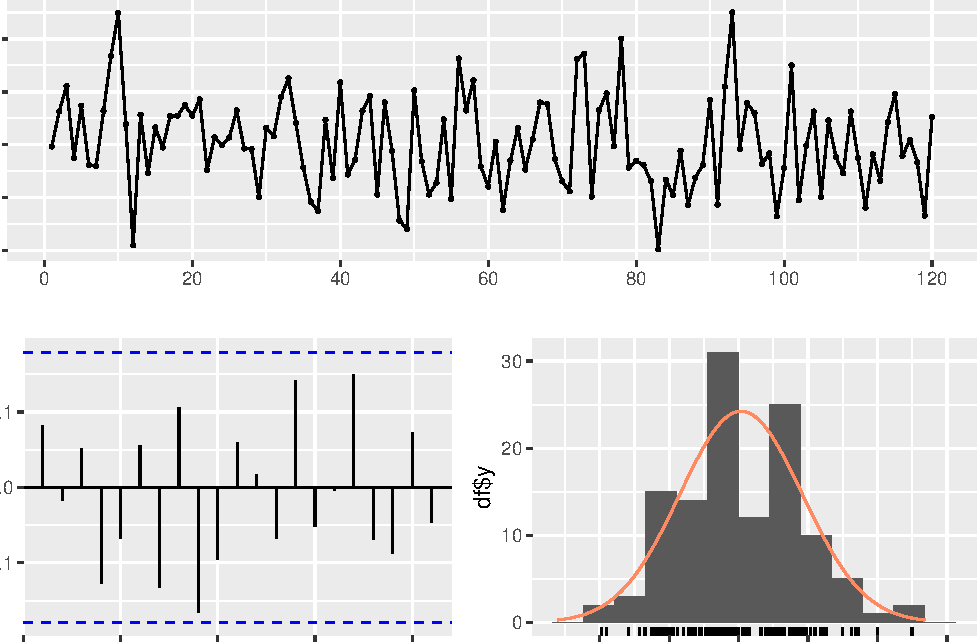
\includegraphics{Bayes_stat_hw2_files/figure-latex/unnamed-chunk-9-1.pdf}

\subsection{8.12}\label{section-5}

\subsubsection{(a)}\label{a-1}

마찬가지로, \(Cauchy(0, 1)\)의 누적분포함수를 구하고, 그 역함수에
\(Unif(0, 1)\)로부터에 난수를 대입한 값은 원래의 분포를 따른다. 코시
분포의 누적분포함수 및 그 역함수는 다음과 같다.

\[
f_X(x) = \frac{1}{\pi(1+x^2)} I\{x \in \mathbb{R}\}
\] \[
F_X(x) = \frac{1}{2} + \frac{1}{\pi} \arctan(x)
\] \[
F_X^{-1}(u) = \tan(\pi(x - \frac{1}{2}))
\]

\subsubsection{(b)}\label{b-1}

\begin{Shaded}
\begin{Highlighting}[]
\FunctionTok{set.seed}\NormalTok{(}\DecValTok{42}\NormalTok{)}
\NormalTok{z }\OtherTok{\textless{}{-}} \FunctionTok{runif}\NormalTok{(}\DecValTok{1000}\NormalTok{, }\DecValTok{0}\NormalTok{, }\DecValTok{1}\NormalTok{)}
\NormalTok{x }\OtherTok{\textless{}{-}} \FunctionTok{tan}\NormalTok{(pi}\SpecialCharTok{*}\NormalTok{(z}\FloatTok{{-}0.5}\NormalTok{))}
\NormalTok{df\_812 }\OtherTok{\textless{}{-}} \FunctionTok{as\_tibble}\NormalTok{(x)}
\end{Highlighting}
\end{Shaded}

\subsubsection{(c)}\label{c-1}

\begin{Shaded}
\begin{Highlighting}[]
\FunctionTok{quantile}\NormalTok{(df\_812}\SpecialCharTok{$}\NormalTok{value, }\FunctionTok{c}\NormalTok{(}\FloatTok{0.25}\NormalTok{, }\FloatTok{0.5}\NormalTok{, }\FloatTok{0.75}\NormalTok{))}
\end{Highlighting}
\end{Shaded}

\begin{verbatim}
##         25%         50%         75% 
## -1.13840874 -0.06183899  0.96264184
\end{verbatim}

한편, 코시 분포에서는 cdf의 역함수가 closed form으로 주어지므로
삼각함수에 대한 방정식을 풀어 백분위를 구할 수 있다. 다음과 같이
백분위수를 구하면 모집단 \(Cauchy(0, 1)\)에서의 백분위수는 다음과 같다.

\[
Ca_{0.25}(0, 1) \; = \; F^{-1}(\frac{1}{4})\; = \; \tan(-\frac{\pi}{4}) \; = \; -1
\]

\[
Ca_{0.5}(0, 1) \; = \; F^{-1}(\frac{1}{2})\; = \; \tan(0) \; = \; 0
\] \[
Ca_{0.75}(0, 1) \; = \; F^{-1}(\frac{3}{4})\; = \; \tan(\frac{\pi}{4}) \; = \; 1
\]

이론상의 백분위수와 사후표본에서의 백분위수가 크게 차이나지 않는 것을
확인할 수 있다.

\subsubsection{(d)}\label{d-1}

\begin{Shaded}
\begin{Highlighting}[]
\FunctionTok{ggplot}\NormalTok{(df\_812, }\FunctionTok{aes}\NormalTok{(}\AttributeTok{x =}\NormalTok{ value)) }\SpecialCharTok{+}
  \FunctionTok{geom\_histogram}\NormalTok{(}\FunctionTok{aes}\NormalTok{(}\AttributeTok{y =} \FunctionTok{after\_stat}\NormalTok{(density)), }\AttributeTok{fill =} \StringTok{"skyblue"}\NormalTok{, }\AttributeTok{alpha =} \FloatTok{0.5}\NormalTok{) }\SpecialCharTok{+}
  \FunctionTok{stat\_function}\NormalTok{(}\AttributeTok{fun =}\NormalTok{ dcauchy, }\AttributeTok{args =} \FunctionTok{list}\NormalTok{(}\AttributeTok{location =} \DecValTok{0}\NormalTok{, }\AttributeTok{scale =} \DecValTok{1}\NormalTok{), }\AttributeTok{color =} \StringTok{"red"}\NormalTok{, }\AttributeTok{n =} \DecValTok{150}\NormalTok{)   }
\end{Highlighting}
\end{Shaded}

\begin{verbatim}
## `stat_bin()` using `bins = 30`. Pick better value with `binwidth`.
\end{verbatim}

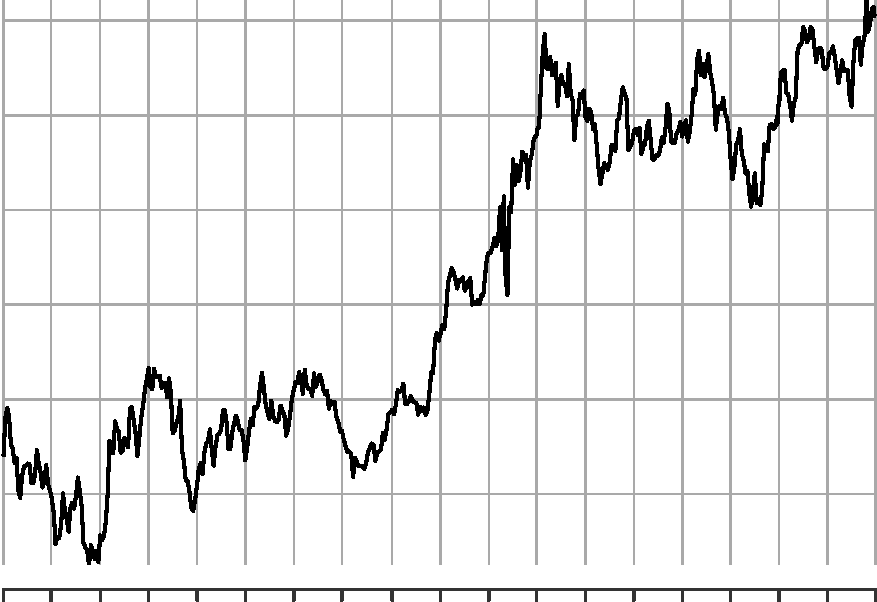
\includegraphics{Bayes_stat_hw2_files/figure-latex/unnamed-chunk-12-1.pdf}

\subsection{8.13}\label{section-6}

\subsubsection{(a)}\label{a-2}

합격-불합격 방법의 구현은 두 단계로 나누어 실행한다. 우선, 한 단계의
합격-불합격 방법을 통해 한 개의 사후표본을 생성하는 함수를 정의한다.
다음으로, \(m\)회 해당 함수를 반복하여 해당 샘플링을 완성하여
데이터프레임에 저장한다.

\begin{Shaded}
\begin{Highlighting}[]
\NormalTok{triangle\_sample }\OtherTok{\textless{}{-}} \ControlFlowTok{function}\NormalTok{()\{}
  \ControlFlowTok{while}\NormalTok{ (}\ConstantTok{TRUE}\NormalTok{) \{}
\NormalTok{    x }\OtherTok{\textless{}{-}} \FunctionTok{runif}\NormalTok{(}\DecValTok{1}\NormalTok{, }\DecValTok{0}\NormalTok{, }\DecValTok{2}\NormalTok{) }\CommentTok{\#제안밀도함수에서 추출 }
\NormalTok{    u }\OtherTok{\textless{}{-}} \FunctionTok{runif}\NormalTok{(}\DecValTok{1}\NormalTok{, }\DecValTok{0}\NormalTok{, }\DecValTok{1}\NormalTok{) }\CommentTok{\#합격 여부 판단을 위한 난수}
\NormalTok{    a }\OtherTok{\textless{}{-}} \FunctionTok{ifelse}\NormalTok{(x }\SpecialCharTok{\textless{}=} \DecValTok{1}\NormalTok{, x, }\DecValTok{2}\SpecialCharTok{{-}}\NormalTok{x) }\CommentTok{\#합격 비율 계산}
    \ControlFlowTok{if}\NormalTok{ (u }\SpecialCharTok{\textless{}=}\NormalTok{ a) \{}
      \FunctionTok{return}\NormalTok{(x)}
\NormalTok{    \}}
\NormalTok{  \}}
\NormalTok{\}}

\FunctionTok{set.seed}\NormalTok{(}\DecValTok{42}\NormalTok{)}
\NormalTok{y }\OtherTok{\textless{}{-}} \FunctionTok{c}\NormalTok{()}
\ControlFlowTok{for}\NormalTok{ (i }\ControlFlowTok{in} \DecValTok{1}\SpecialCharTok{:}\DecValTok{1000}\NormalTok{) \{}
\NormalTok{  y }\OtherTok{\textless{}{-}} \FunctionTok{append}\NormalTok{(y, }\FunctionTok{triangle\_sample}\NormalTok{())}
\NormalTok{\}}
\NormalTok{df\_813 }\OtherTok{\textless{}{-}} \FunctionTok{as\_tibble}\NormalTok{(y)}
\end{Highlighting}
\end{Shaded}

\subsubsection{(b)}\label{b-2}

\begin{Shaded}
\begin{Highlighting}[]
\FunctionTok{mean}\NormalTok{(df\_813}\SpecialCharTok{$}\NormalTok{value)}
\end{Highlighting}
\end{Shaded}

\begin{verbatim}
## [1] 0.9958629
\end{verbatim}

\begin{Shaded}
\begin{Highlighting}[]
\FunctionTok{sd}\NormalTok{(df\_813}\SpecialCharTok{$}\NormalTok{value)}
\end{Highlighting}
\end{Shaded}

\begin{verbatim}
## [1] 0.4063675
\end{verbatim}

이론적으로 \(xI\{0\leq x \leq 1\} \; + \; (2-x)I\{1 < x \leq 2\}\)와
같이 정의된 삼각분포의 평균은 1, 표준편차는 \(\frac{1}{\sqrt6}\)이다.
이와 같은 이론적 값과 실제 분포상 값 0.9958629, 0.4063675가 유사함을
확인할 수 있다.

\subsubsection{(c)}\label{c-2}

\begin{Shaded}
\begin{Highlighting}[]
\NormalTok{tri\_pdf }\OtherTok{\textless{}{-}} \ControlFlowTok{function}\NormalTok{(x) \{}
  \FunctionTok{ifelse}\NormalTok{(x }\SpecialCharTok{\textgreater{}=} \DecValTok{0} \SpecialCharTok{\&}\NormalTok{ x }\SpecialCharTok{\textless{}=} \DecValTok{1}\NormalTok{, x,}
         \FunctionTok{ifelse}\NormalTok{(x }\SpecialCharTok{\textgreater{}} \DecValTok{1} \SpecialCharTok{\&}\NormalTok{ x }\SpecialCharTok{\textless{}=} \DecValTok{2}\NormalTok{, }\DecValTok{2} \SpecialCharTok{{-}}\NormalTok{ x, }\DecValTok{0}\NormalTok{))}
\NormalTok{\}}

\FunctionTok{ggplot}\NormalTok{(df\_813, }\FunctionTok{aes}\NormalTok{(}\AttributeTok{x =}\NormalTok{ value)) }\SpecialCharTok{+}
  \FunctionTok{geom\_histogram}\NormalTok{(}\FunctionTok{aes}\NormalTok{(}\AttributeTok{y =} \FunctionTok{after\_stat}\NormalTok{(density)), }\AttributeTok{fill =} \StringTok{"skyblue"}\NormalTok{, }\AttributeTok{alpha =} \FloatTok{0.5}\NormalTok{) }\SpecialCharTok{+}
  \FunctionTok{stat\_function}\NormalTok{(}\AttributeTok{fun =}\NormalTok{ tri\_pdf, }\AttributeTok{color =} \StringTok{"red"}\NormalTok{)}
\end{Highlighting}
\end{Shaded}

\begin{verbatim}
## `stat_bin()` using `bins = 30`. Pick better value with `binwidth`.
\end{verbatim}

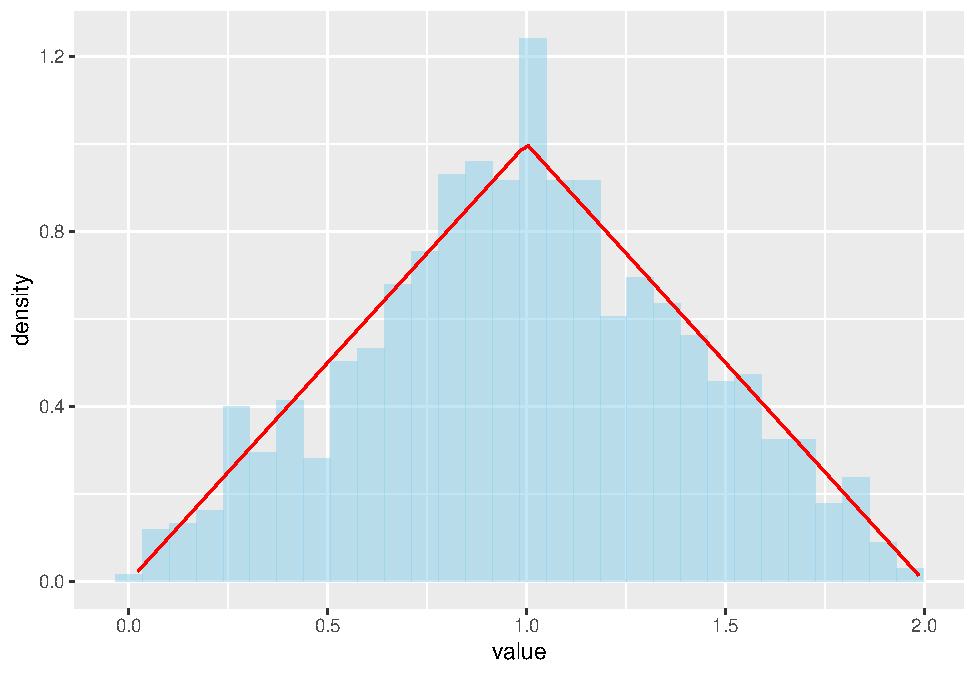
\includegraphics{Bayes_stat_hw2_files/figure-latex/unnamed-chunk-15-1.pdf}

\subsection{8.14}\label{section-7}

\subsubsection{(a)}\label{a-3}

다음과 같이 코시 분포를 제안분포로 하여 1개의 정규확률변수를 생성하는
함수를 정의한다.

\begin{Shaded}
\begin{Highlighting}[]
\NormalTok{normal\_sample }\OtherTok{\textless{}{-}} \ControlFlowTok{function}\NormalTok{()\{}
\NormalTok{  M }\OtherTok{\textless{}{-}} \DecValTok{2}\SpecialCharTok{/}\FunctionTok{sqrt}\NormalTok{(}\FunctionTok{exp}\NormalTok{(}\DecValTok{1}\NormalTok{)) }\CommentTok{\# 봉투상수}
  \ControlFlowTok{while}\NormalTok{ (}\ConstantTok{TRUE}\NormalTok{) \{}
\NormalTok{    x }\OtherTok{\textless{}{-}} \FunctionTok{rcauchy}\NormalTok{(}\DecValTok{1}\NormalTok{, }\DecValTok{0}\NormalTok{, }\DecValTok{1}\NormalTok{) }\CommentTok{\#제안밀도함수에서 추출 }
\NormalTok{    u }\OtherTok{\textless{}{-}} \FunctionTok{runif}\NormalTok{(}\DecValTok{1}\NormalTok{, }\DecValTok{0}\NormalTok{, }\DecValTok{1}\NormalTok{) }\CommentTok{\#합격 여부 판단을 위한 난수}
\NormalTok{    a }\OtherTok{\textless{}{-}}\NormalTok{ (}\DecValTok{1}\SpecialCharTok{+}\NormalTok{x}\SpecialCharTok{\^{}}\DecValTok{2}\NormalTok{)}\SpecialCharTok{*}\FunctionTok{exp}\NormalTok{(}\SpecialCharTok{{-}}\NormalTok{(x}\SpecialCharTok{\^{}}\DecValTok{2}\NormalTok{)}\SpecialCharTok{/}\DecValTok{2}\NormalTok{)}\SpecialCharTok{/}\NormalTok{M }\CommentTok{\#합격 비율 계산}
    \ControlFlowTok{if}\NormalTok{ (u }\SpecialCharTok{\textless{}=}\NormalTok{ a) \{}
      \FunctionTok{return}\NormalTok{(x)}
\NormalTok{    \}}
\NormalTok{  \}}
\NormalTok{\}}
\end{Highlighting}
\end{Shaded}

이제 위의 함수를 이용하여 1000개의 정규확률변수를 생성한다.

\begin{Shaded}
\begin{Highlighting}[]
\FunctionTok{set.seed}\NormalTok{(}\DecValTok{42}\NormalTok{)}
\NormalTok{y }\OtherTok{\textless{}{-}} \FunctionTok{c}\NormalTok{()}
\ControlFlowTok{for}\NormalTok{ (i }\ControlFlowTok{in} \DecValTok{1}\SpecialCharTok{:}\DecValTok{1000}\NormalTok{) \{}
\NormalTok{  y }\OtherTok{\textless{}{-}} \FunctionTok{append}\NormalTok{(y, }\FunctionTok{normal\_sample}\NormalTok{())}
\NormalTok{\}}
\NormalTok{df\_814 }\OtherTok{\textless{}{-}} \FunctionTok{as\_tibble}\NormalTok{(y)}
\end{Highlighting}
\end{Shaded}

\subsubsection{(b)}\label{b-3}

\begin{Shaded}
\begin{Highlighting}[]
\FunctionTok{mean}\NormalTok{(df\_814}\SpecialCharTok{$}\NormalTok{value)}
\end{Highlighting}
\end{Shaded}

\begin{verbatim}
## [1] 0.0437004
\end{verbatim}

\begin{Shaded}
\begin{Highlighting}[]
\FunctionTok{sd}\NormalTok{(df\_814}\SpecialCharTok{$}\NormalTok{value)}
\end{Highlighting}
\end{Shaded}

\begin{verbatim}
## [1] 0.9954824
\end{verbatim}

표준정규분포 \(N(0, 1^2)\)의 평균은 0, 표준편차는 1이므로 사후평균
0.0437004, 사후표준편차 0.9954824와 유사하다.

\subsubsection{(c)}\label{c-3}

\begin{Shaded}
\begin{Highlighting}[]
\FunctionTok{ggplot}\NormalTok{(df\_814, }\FunctionTok{aes}\NormalTok{(}\AttributeTok{x =}\NormalTok{ value)) }\SpecialCharTok{+}
  \FunctionTok{geom\_histogram}\NormalTok{(}\FunctionTok{aes}\NormalTok{(}\AttributeTok{y =} \FunctionTok{after\_stat}\NormalTok{(density)), }\AttributeTok{fill =} \StringTok{"skyblue"}\NormalTok{, }\AttributeTok{alpha =} \FloatTok{0.5}\NormalTok{) }\SpecialCharTok{+}
  \FunctionTok{stat\_function}\NormalTok{(}\AttributeTok{fun =}\NormalTok{ dnorm, }\AttributeTok{args =} \FunctionTok{list}\NormalTok{(}\AttributeTok{mean =} \DecValTok{0}\NormalTok{, }\AttributeTok{sd =} \DecValTok{1}\NormalTok{), }\AttributeTok{color =} \StringTok{"red"}\NormalTok{) }
\end{Highlighting}
\end{Shaded}

\begin{verbatim}
## `stat_bin()` using `bins = 30`. Pick better value with `binwidth`.
\end{verbatim}

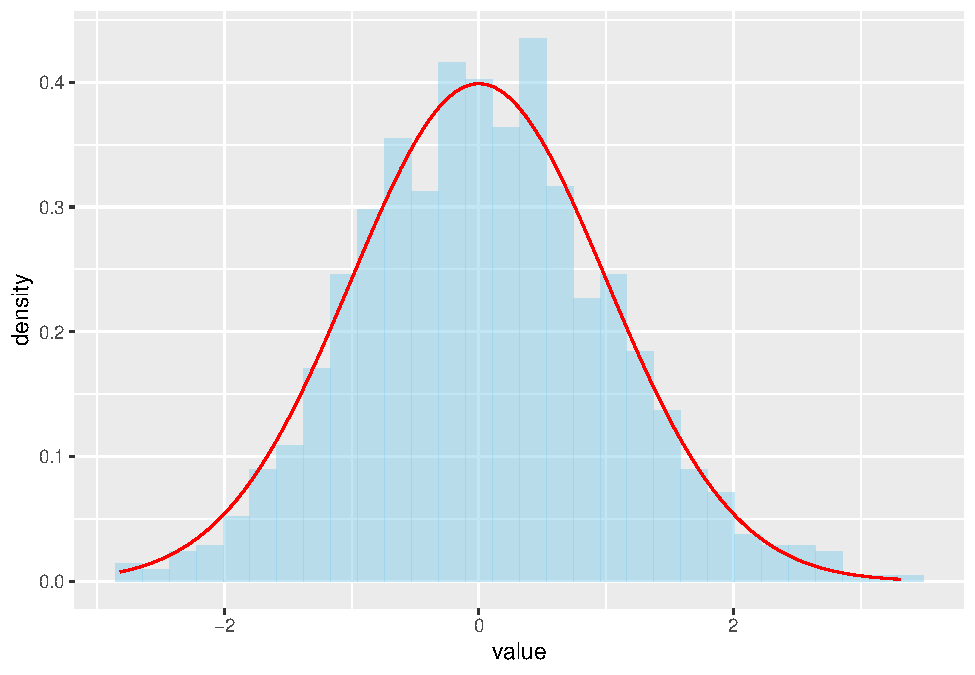
\includegraphics{Bayes_stat_hw2_files/figure-latex/unnamed-chunk-19-1.pdf}

\subsection{8.15}\label{section-8}

\subsubsection{(a)}\label{a-4}

박스-뮐러 변환을 통한 정규확률변수 생성은 두 단계로 구성된다. 우선,
\((u1, u2) \;{\sim}\; Unif((0, 1)^2)\)를 생성할 수 있으므로 이로부터
적절한 지수분포와 균등분포를 생성할 수 있다. 다음으로, 서로 독립인 이
지수분포와 균등분포를 극좌표계 표현을 통해 조합함으로써 서로 독립인
정규확률변수를 생성할 수 있다.

코드의 u1, u2는 균등분포를 따르는 랜덤 확률변수를 생성하는 부분이고, v와
t는 이와 같이 생성된 균등분포로부터 지수분포, 균등분포를 따르는 서로
독립인 적절한 확률분포(또는 확률분포의 상수배)를 생성하는 과정이며, 세
번째 x1, x2는 지수분포와 균등분포의 함수로써 생성된 이변량 정규분포 x1,
x2의 좌표이다.

\begin{Shaded}
\begin{Highlighting}[]
\FunctionTok{set.seed}\NormalTok{(}\DecValTok{42}\NormalTok{)}
\NormalTok{u1 }\OtherTok{\textless{}{-}} \FunctionTok{runif}\NormalTok{(}\DecValTok{1000}\NormalTok{, }\DecValTok{0}\NormalTok{, }\DecValTok{1}\NormalTok{)}
\NormalTok{u2 }\OtherTok{\textless{}{-}} \FunctionTok{runif}\NormalTok{(}\DecValTok{1000}\NormalTok{, }\DecValTok{0}\NormalTok{, }\DecValTok{1}\NormalTok{)}
\NormalTok{v }\OtherTok{\textless{}{-}} \SpecialCharTok{{-}}\DecValTok{2}\SpecialCharTok{*}\FunctionTok{log}\NormalTok{(}\DecValTok{1}\SpecialCharTok{{-}}\NormalTok{u1) }\CommentTok{\#transform (u1, u2) to (v, t)}
\NormalTok{t }\OtherTok{\textless{}{-}} \DecValTok{2}\SpecialCharTok{*}\NormalTok{pi}\SpecialCharTok{*}\NormalTok{u2}
\NormalTok{x1 }\OtherTok{\textless{}{-}} \FunctionTok{sqrt}\NormalTok{(v)}\SpecialCharTok{*}\FunctionTok{cos}\NormalTok{(t) }\CommentTok{\#transform (v, t) to (x1, x2)}
\NormalTok{x2 }\OtherTok{\textless{}{-}} \FunctionTok{sqrt}\NormalTok{(v)}\SpecialCharTok{*}\FunctionTok{sin}\NormalTok{(t)}
\NormalTok{df\_815 }\OtherTok{\textless{}{-}} \FunctionTok{data.frame}\NormalTok{(x1, x2) }\CommentTok{\#save bivariate normal distribution (x1, x2)}
\end{Highlighting}
\end{Shaded}

\subsubsection{(b)}\label{b-4}

\begin{Shaded}
\begin{Highlighting}[]
\FunctionTok{colMeans}\NormalTok{(df\_815) }
\end{Highlighting}
\end{Shaded}

\begin{verbatim}
##          x1          x2 
##  0.04197130 -0.01846759
\end{verbatim}

\begin{Shaded}
\begin{Highlighting}[]
\FunctionTok{var}\NormalTok{(df\_815)}
\end{Highlighting}
\end{Shaded}

\begin{verbatim}
##             x1          x2
## x1  0.97851484 -0.01314774
## x2 -0.01314774  0.94863882
\end{verbatim}

\begin{Shaded}
\begin{Highlighting}[]
\FunctionTok{sd}\NormalTok{(df\_815}\SpecialCharTok{$}\NormalTok{x1)}
\end{Highlighting}
\end{Shaded}

\begin{verbatim}
## [1] 0.9891991
\end{verbatim}

\begin{Shaded}
\begin{Highlighting}[]
\FunctionTok{sd}\NormalTok{(df\_815}\SpecialCharTok{$}\NormalTok{x2)}
\end{Highlighting}
\end{Shaded}

\begin{verbatim}
## [1] 0.9739809
\end{verbatim}

표본 1000개의 평균과 표준편차는 위와 같다. 이때, 이변량 정규분포의
평균벡터는 \(\begin{pmatrix}0\\0\end{pmatrix}\)이고 분산행렬은
\(\begin{pmatrix}1&0\\0&1\end{pmatrix}\)이다. 물론 x1, x2 각각
표준편차는 1이다. 박스-뮐러 변환을 통해 생성된 표준편차들 (0.9891991,
0.9739809)과과 이론상 값이 큰 차이가 없는 것을 확인 가능하다.

\subsubsection{(c)}\label{c-4}

\begin{Shaded}
\begin{Highlighting}[]
\FunctionTok{ggplot}\NormalTok{(df\_815, }\FunctionTok{aes}\NormalTok{(}\AttributeTok{x =}\NormalTok{ x1)) }\SpecialCharTok{+}
  \FunctionTok{geom\_histogram}\NormalTok{(}\FunctionTok{aes}\NormalTok{(}\AttributeTok{y =} \FunctionTok{after\_stat}\NormalTok{(density)), }\AttributeTok{fill =} \StringTok{"skyblue"}\NormalTok{, }\AttributeTok{alpha =} \FloatTok{0.5}\NormalTok{) }\SpecialCharTok{+}
  \FunctionTok{stat\_function}\NormalTok{(}\AttributeTok{fun =}\NormalTok{ dnorm, }\AttributeTok{args =} \FunctionTok{list}\NormalTok{(}\AttributeTok{mean =} \DecValTok{0}\NormalTok{, }\AttributeTok{sd =} \DecValTok{1}\NormalTok{), }\AttributeTok{color =} \StringTok{"red"}\NormalTok{) }
\end{Highlighting}
\end{Shaded}

\begin{verbatim}
## `stat_bin()` using `bins = 30`. Pick better value with `binwidth`.
\end{verbatim}

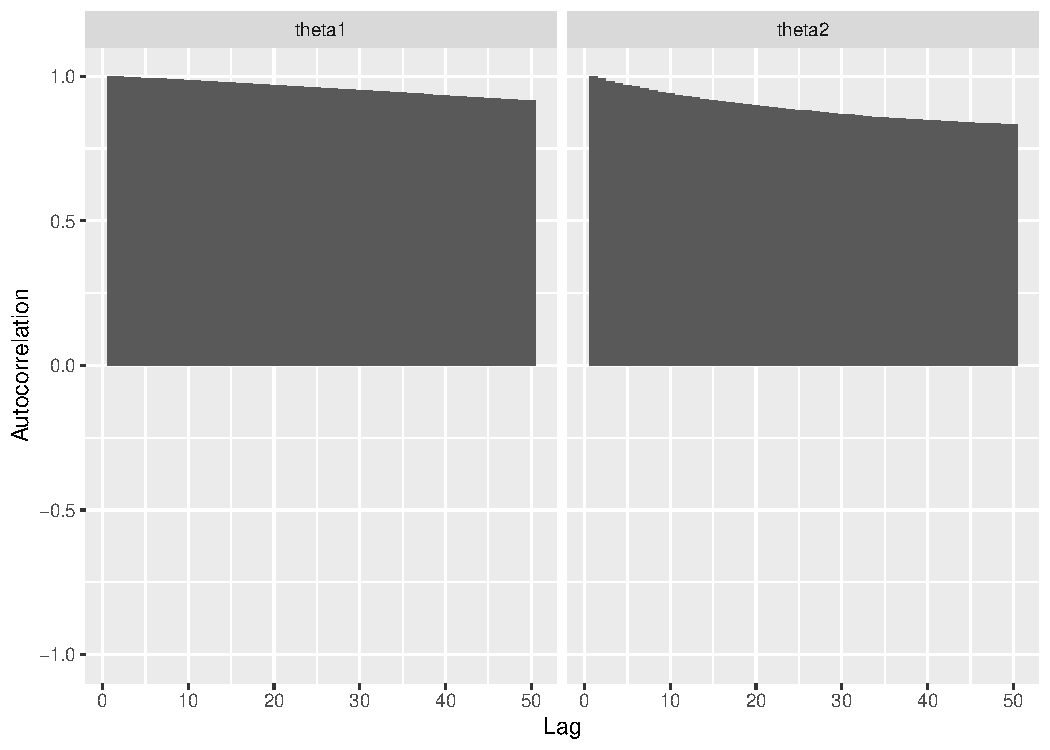
\includegraphics{Bayes_stat_hw2_files/figure-latex/unnamed-chunk-22-1.pdf}

\begin{Shaded}
\begin{Highlighting}[]
\FunctionTok{ggplot}\NormalTok{(df\_815, }\FunctionTok{aes}\NormalTok{(}\AttributeTok{x =}\NormalTok{ x2)) }\SpecialCharTok{+}
  \FunctionTok{geom\_histogram}\NormalTok{(}\FunctionTok{aes}\NormalTok{(}\AttributeTok{y =} \FunctionTok{after\_stat}\NormalTok{(density)), }\AttributeTok{fill =} \StringTok{"skyblue"}\NormalTok{, }\AttributeTok{alpha =} \FloatTok{0.5}\NormalTok{) }\SpecialCharTok{+}
  \FunctionTok{stat\_function}\NormalTok{(}\AttributeTok{fun =}\NormalTok{ dnorm, }\AttributeTok{args =} \FunctionTok{list}\NormalTok{(}\AttributeTok{mean =} \DecValTok{0}\NormalTok{, }\AttributeTok{sd =} \DecValTok{1}\NormalTok{), }\AttributeTok{color =} \StringTok{"red"}\NormalTok{) }
\end{Highlighting}
\end{Shaded}

\begin{verbatim}
## `stat_bin()` using `bins = 30`. Pick better value with `binwidth`.
\end{verbatim}

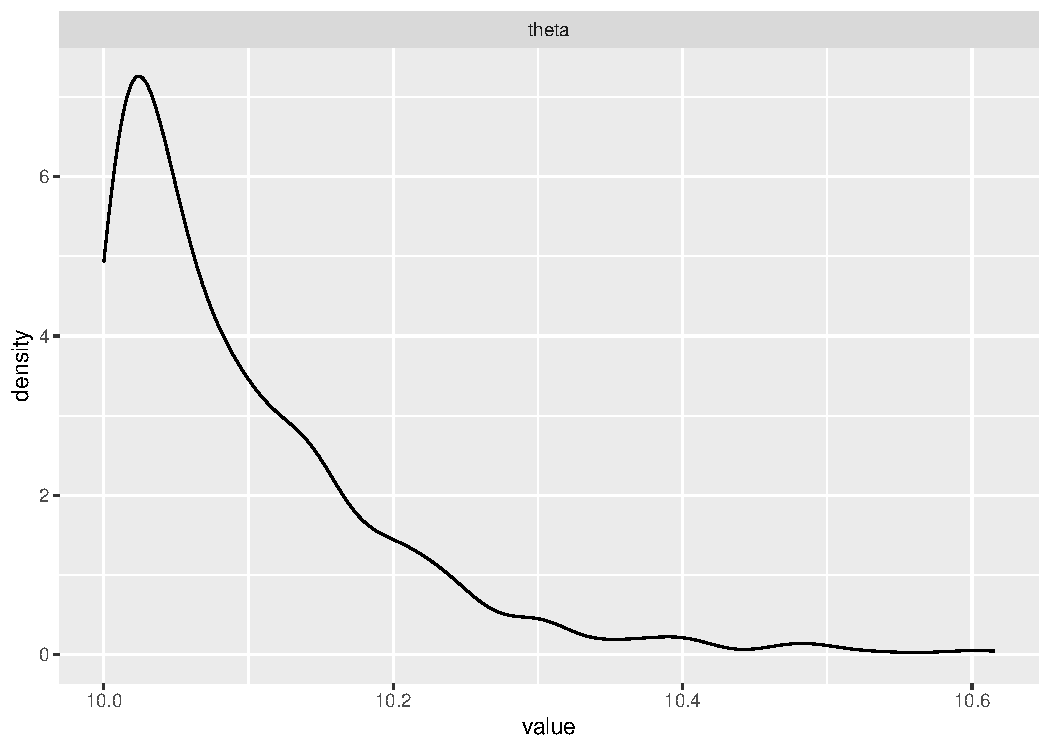
\includegraphics{Bayes_stat_hw2_files/figure-latex/unnamed-chunk-23-1.pdf}

\end{document}
